\chapter{The Normalization Channel \texorpdfstring{\decay{\Lb}{\Dz\proton\pim}}{Λb → Dpπ}}
\label{chap:norm}
A normalization channel should comprise two key characteristics: First, the decay topology should be as close as possible to the primary decay channel such that common uncertainties and biases cancel.
Secondly, the normalization channel should be well established, clean to extract and contribute to the error budget as little as possible.

Obvious candidates for the present analysis are \decay{\Lb}{\Dz\proton\pim}, \decay{\Lb}{\Lz\Kp\pim}, \decay{\Lb}{\jpsi\Lz} and \decay{\Bbar{}^0_{(\squark)}}{\Dzb\KS}.
Despite its large branching fraction and clean reconstruction, the \jpsi\Lz mode, in particular if the \jpsi is reconstructed in its dimuon mode, will differ strongly in its detector response and trigger signature and thus requires a careful study of the corresponding simulation fidelity of both modes and therefore is not an ideal candidate.
The branching fractions of the other modes, as reported by the \gls{pdg}, are
\begin{align*}
    \BR(\decay{\Lb}{\Dz\proton\pim}) &= (6.3 \pm 0.7) \times 10^{-4} \,, \\
    \BR(\decay{\Lb}{\Lz\Kp\pim}) &= (5.7 \pm 1.3) \times 10^{-6} \,, \\
    \BR(\decay{\Bd}{\Dzb\Kz}) &= (5.2 \pm 0.7) \times 10^{-5} \,, \\
    \BR(\decay{\Bs}{\Dzb\Kzb}) &= (4.3 \pm 0.9) \times 10^{-4} \,,
\end{align*}
which do not include the \bquark-hadron production fractions which themselves depend on the kinematics of the \bquark~quark~\cite{LHCb_bProdFrac_7,LHCb_bProdFrac_13}.
Further, only roughly half of the \Kz mesons decay as \KS and within a similar detector acceptance as \Lz baryons.\footnote{Neglecting small \CP{} violating corrections and assuming similar lifetimes of the \KS state and the \Lz baryon.}
The other part will most likely escape undetected.
Taking both effects into account qualifies \decay{\Lb}{\Dz\proton\pim} as the most efficient candidate.

The final states of the charmless three-body decay approximate the signature of \decay{\Lb}{\Dz\Lz} best, but this advantage is compensated by its small branching fraction and the noisy background (\cf{}~Ref.~\cite{LbToLzhh}).
We note that this valuation will likely change in the future and future experiments might rank charmless three-body decays as their most suitable normalization candidate if provided with a sufficiently large set of \Lb decays.

The listed \bquark-meson decays also have a long living $\PV^0$ particle in their decay chain.
During analysis, \decay{\KS}{\pip\pim} decays have to be grouped w.r.t.\ their track types \gls{LL} and \gls{DD}, similar to \decay{\Lz}{\proton\pim}.
On the one hand, this leverages the access to track type specific properties which could cancel partially in the branching ratio, on the other hand, splitting the data sample hampers the analysis and, even though \KS and \Lz are both $\PV^0$ particles, the final states \pip\pim and \proton\pim can cause different signatures in the \lhcb{} detector which make \Dz\proton\pim the better proxy for \Dz\Lz, especially for \gls{LL} tracks.
At the same time, the fidelity of \gls{mc} simulated \Lb decays is known for being imperfect, especially in terms of kinematic distributions.
Using \Lb decays in the primary decay, as well as the normalization mode minimizes this uncertainty source in the branching fraction.

Considering the listed arguments, we use \decay{\Lb}{\Dz\proton\pim} as the normalization mode.
We will briefly discuss the decay in Sec.~\ref{sec:LbToDzppi_thedecay} and will then outline the selection strategy.
In Sec.~\ref{sec:LbToDzppi_yields} we will then extract signal yields which we will use later for determining the branching fraction.

\section{The Decay \texorpdfstring{\decay{\Lb}{\Dz\proton\pim}}{Λb → Dpπ}}
\label{sec:LbToDzppi_thedecay}
The decay \decay{\Lb}{\Dz\proton\pim} is a high statistics channel and leveraged the discovery of the \Lb baryon in 1981 \cite{Lbdisc}.
The final states are the same as in \decay{\Lb}{\Dz\Lz} but due to the different quark transitions, it is much less susceptible for \CP violation.\footnote{Changing the pion to a kaon reduces the branching fraction by a factor of $\lambda^2$ (\gls{wolfenstein}) but now allows an effective extraction of the \gls{ckm} phase $\gamma$ (\cf{} Sec.~\ref{sec:lbcpv}).} 
The large branching fraction gives a good signal to background ratio after applying simple rectangular selection requirements.
Rather than optimizing these selection requirements for \decay{\Lb}{\Dz\proton\pim}, the opulent signal to background ratio allows the use of a subset of the optimized requirements for the primary decay \decay{\Lb}{\Dz\Lz} with some minor corrections. 
These selections are split into a preselection and a loose selection part which are outlined in the following sections.

\subsection{Preselection}
We use the full recorded data set of \gls{runtwo} and the \gls{stripping} versions listed in Tab.~\ref{tab:LbToDzLz_vstripping}.
Despite their different naming, the selection requirements vary slightly.
These differences are compensated by adopting the tightest selection requirement among conflicting values if necessary.

\begin{table}[htbp]
    \centering
    \caption{\Gls{stripping} and Reco versions used for reconstructing \decay{\Lb}{\Dz\proton\pim}.}
    \label{tab:LbToDzppi_vstripping}

    \begin{tabular}{lll}
        \toprule
        Year & \Gls{stripping} & Reco \\
        \midrule
        2015 & \texttt{24r1} & \texttt{15a} \\
        2016 & \texttt{28r1} & \texttt{16} \\
        2017 & \texttt{29r2} & \texttt{17} \\
        2018 & \texttt{34} & \texttt{18} \\
        \bottomrule
    \end{tabular}
\end{table}

All selection criteria of the preselection step are listed in Tab.~\ref{tab:LbToDzppi_stripsel} where we use the same nomenclature that we introduced in Sec.~\ref{sec:LbToJpsiLz_presel}.
Additionally, at least one \gls{hlt} trigger flag among \texttt{Hlt2.*IncPhi.*Decision} or \texttt{Hlt2Topo.*Decision} is required, \cf{}~Refs.~\cite{triggerRun2,HTL2TopoLines} for more detailed information.

\subsection{Loose Selection}
\label{sec:LbToDzppi_loosesel}
Similar to the previous analyses of \decay{\Lb}{\jpsi\Lz} and \decay{\Lb}{\Dz\Lz} decays, we select only events corresponding to the best \gls{pv} hypothesis for the following steps.
All selection criteria of the loose selection are shown in Tab.~\ref{tab:LbToDzppi_loosesel} and are grouped into five categories.
Again, categories~1 to 4 are the same that we used and described previously in Sec.~\ref{sec:LbToJpsiLz_loosesel} and Sec.~\ref{sec:LbToDzLz_loosesel}.
The purpose of selection requirements of category~5 is to reject physical backgrounds such as \decay{\Bd}{\Dzb\pip\pim}, \decay{\Bd}{\Dzb\Km\pip} or \decay{\Bs}{\Dzb\Km\pip} and \decay{\Lb}{\Dz\proton\Km} by requiring a minimal threshold w.r.t.\ $\texttt{ProbNNp}(\proton)$ and a veto against large values of $\texttt{ProbNNk}(\pion)$, respectively.
Since most of the charge tracks in an event are caused by genuine pions, the former selection requirement also helps to suppress combinatorial background (category~1).
The combined efficiency for \gls{mc} simulated events is $71.10(25)\,\%$ where the uncertainty only takes statistical fluctuations into account (\cf{}~Sec.~\ref{sec:LbToDzLz_loosesel}).

\begin{table}[htbp]
    \caption{Selection criteria of loose selection used for reconstructing \decay{\Lb}{\Dz\proton\pim}. The selections are grouped into four categories which are explained in Sec.~\ref{sec:LbToDzppi_loosesel}.}
    \label{tab:LbToDzppi_loosesel}
    \centering
    \begin{tabular}{llc}
        \toprule
        Particle & Selection & Category \\
        \midrule
        \pion & $3 \le p \le 150\,$\gevc & 1 \\
        \kaon & $3 \le p \le 150\,$\gevc & 1 \\
        \proton & $9 \le p \le 150\,$\gevc & 1 \\
        \proton & \texttt{ProbNNp} $\ge 0.2$ & 1, 5 \\
        \pi & \texttt{ProbNNk} $\le 0.3$ & 5 \\
        \midrule
        \Dz & $0 \le$ FD sig. $\le 100$ & 1 \\
        \Dz & \dchisqip w.r.t.\ best \gls{pv} $\ge 5$ & 1 \\
        \midrule
        \Lb & \dchisqip w.r.t.\ best \gls{pv} $\le 25$ & 1 \\
        \Lb & $5 \le m \le 6\,\gevcc$ & 3 \\
        \Lb & $2 \le \eta \le 4.5$ & 4 \\
        \Lb & $\pt \le 20\,\gevc$ & 4 \\
        \midrule
        \Lb & $\exists$ converged \gls{dtf} & 1 \\
        \Lb & $\chi_\mathrm{DTF}^2 / \text{\gls{dof}} \le 10$ & 1 \\
        \bottomrule
    \end{tabular}
\end{table}

\subsection{Calibration}
\label{sec:norm_calibration}
Three-body decays typically have resonances among their final states, whereas in two-body decays the only possible resonance is the mother of the decay chain itself.
In particular, \decay{\Lb}{\Dz\proton\pim} decays have a rich set of resonances among \Dz\proton and \Dz\pim pairs~\cite{LbToDzphAndLch}.
These resonances are not taken into account during the generation of the \gls{mc} simulated decays.
Instead, the decays are simulated flat in the so-called \textit{square Dalitz plot} (\cf{} Refs.~\cite{dalitz1,dalitz2} and in particular Ref.~\cite{BsToDKpi} for the definition of a square Dalitz plot).
In order to make recorded data and \gls{mc} simulated event comparable we calibrate the former by assigning weights to each event.\footnote{Technically, the parameters $m'$ and $\theta'$ (\cf{}~Ref.~\cite{BsToDKpi}), are evaluated with a \Gls{dtf} where all intermediate particle masses (\ie{}, including $m(\Lb)$ itself) are constrained to increase the resolution of the Dalitz distribution.}
The weights are the inverted values of the (normalized) smoothed square Dalitz plot profile, where the smoothing is performed in bins using a $5 \times 5$ kernel function
\begin{equation*}
    \mathcal{K} = \begin{pmatrix}
        0 & 0 & 1 & 0 & 0 \\
        0 & 2 & 2 & 2 & 0 \\
        1 & 2 & 5 & 2 & 1 \\
        0 & 2 & 2 & 2 & 0 \\
        0 & 0 & 1 & 0 & 0
    \end{pmatrix}.
\end{equation*}
The smoothed profile is the result of a convolution with $\mathcal{K}$ and a subsequent normalization where kernel pixels that extends past the boundary are set to zero (Kernel Crop).
Below, we apply this efficiency correction to recorded data after the respective selection steps but suppress an explicit mention for the sake of brevity.
As a consequence, we also use (binned) weighted minimum $\chi^2$-fits in the following instead of a (single entry) maximum likelihood method.
Calibrating the recorded data changes the shapes of the physical background, whereas the impact on the fitted signal yields is less than $14\,\%$.

\section{Yield Extraction}
\label{sec:LbToDzppi_yields}
The distribution of the invariant mass $m(\Dz\proton\pim)$ after applying the loose selection requirements is shown in Fig.~\ref{fig:LbToDzppi_mLb_nocuts}.
\begin{figure}[htbp]
    \centering
    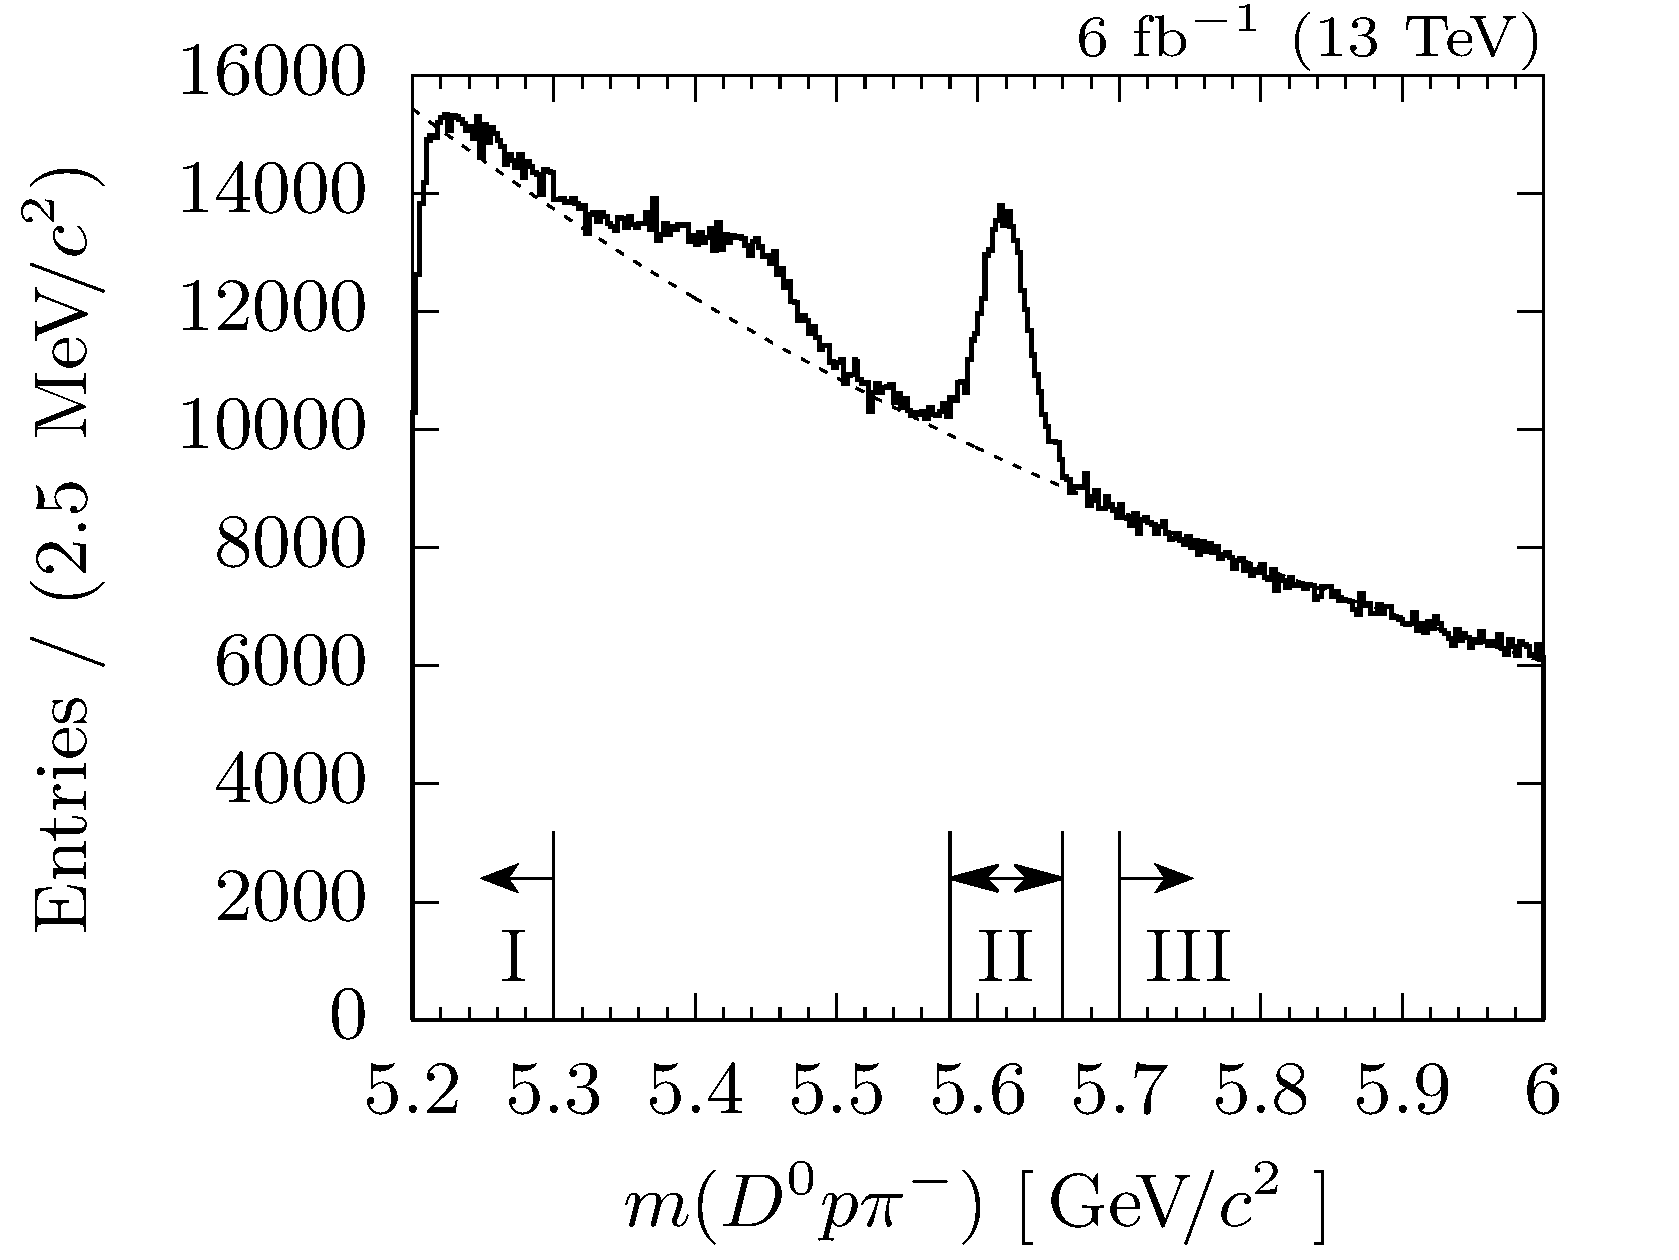
\includegraphics[scale=1.]{Lb2Dzppi_mvaxcheck/mLb_nocuts.png}
    \caption{Invariant mass distribution of \Dz, \proton and \pim candidates after applying the loose selection requirements. The regions I and III are used for extracting the shape of the combinatorial background. Region II indicates the signal region that is used for extracting the signal yield. The dashed line indicate the fitted shape of the combinatorial background.}
    \label{fig:LbToDzppi_mLb_nocuts}
\end{figure}
An exhaustive fit model that comprises a precise signal model, as well as all background components such as partially reconstructed \decay{\Lb}{\Dstarz\proton\pim} (large enhancement between $5.3\,\gevcc$ and $5.5\,\gevcc$) or \glspl{reflection} from \decay{\Lb}{\Dz\proton\Km} decays or other \Bd and \Bs decays requires a thorough analysis of all these components, \cf{}~Ref.~\cite{LbToDzphAndLch}.
For the present analysis we find that a simple yet flexible fit model suffices, while not contributing to the overall error budget excessively.
Within this fit model, the signal region is limited tightly to $5.58 \le m(\Dz\proton\pim) \le 5.66\,\gevcc$ (region II in Fig.~\ref{fig:LbToDzppi_mLb_nocuts}) and thus reduces the impact of physical background contribution, in particular of \glspl{reflection} below $m(\Lb)$.
The shape of the combinatorial background is parametrized with the exponential function given in Eq.~\eqref{eq:apdx_pdfs_exprel2} and is extracted from a lower sideband $5.2 \le m(\Dz\proton\pim) \le 5.3\,\gevcc$ and an upper sideband $5.7 \le m(\Dz\proton\pim) \le 6\,\gevcc$, referred to as region I and III in Fig.~\ref{fig:LbToDzppi_mLb_nocuts}.
The signal yield is obtained by extrapolating the fitted background \gls{pdf} into region~II, scaling with the number of events in regions~I and III, and subtracting the result from the number of events in region~II.
Applying this fitting strategy to the distribution of the invariant mass $m(\Dz\proton\pim)$ after the loose selection, as shown in Fig.~\ref{fig:LbToDzppi_mLb_nocuts}, yields $7.04(6) \times 10^4$ signal events where the uncertainty only takes statistical fluctuations into account.
In order to estimate the systematic uncertainty we use the same fitting strategy to extract the yields from two further reduced samples, where the former (latter) sample is obtained by requiring $\texttt{ProbNNk} \ge 0.3$ ($0.57$) for the kaon and a \gls{dtf} probability above $0.01$.
The thresholds of the selection requirements w.r.t.\ the \texttt{ProbNNk} responses are the optimized values for \gls{LL} and \gls{DD} tracks that we found for the \decay{\Lb}{\Dz\Lz} decay in Chap.~\ref{chap:mva}, whereas the threshold w.r.t.\ the \gls{dtf} probability is chosen ad hoc and proven to significantly improve the signal to background ratio.
Both samples are shown in Fig.~\ref{fig:LbToDzppi_hLbM_no_clf}.
\begin{figure}[htbp]
    \centering
    \begin{subfigure}{.49\textwidth}
        \centering
        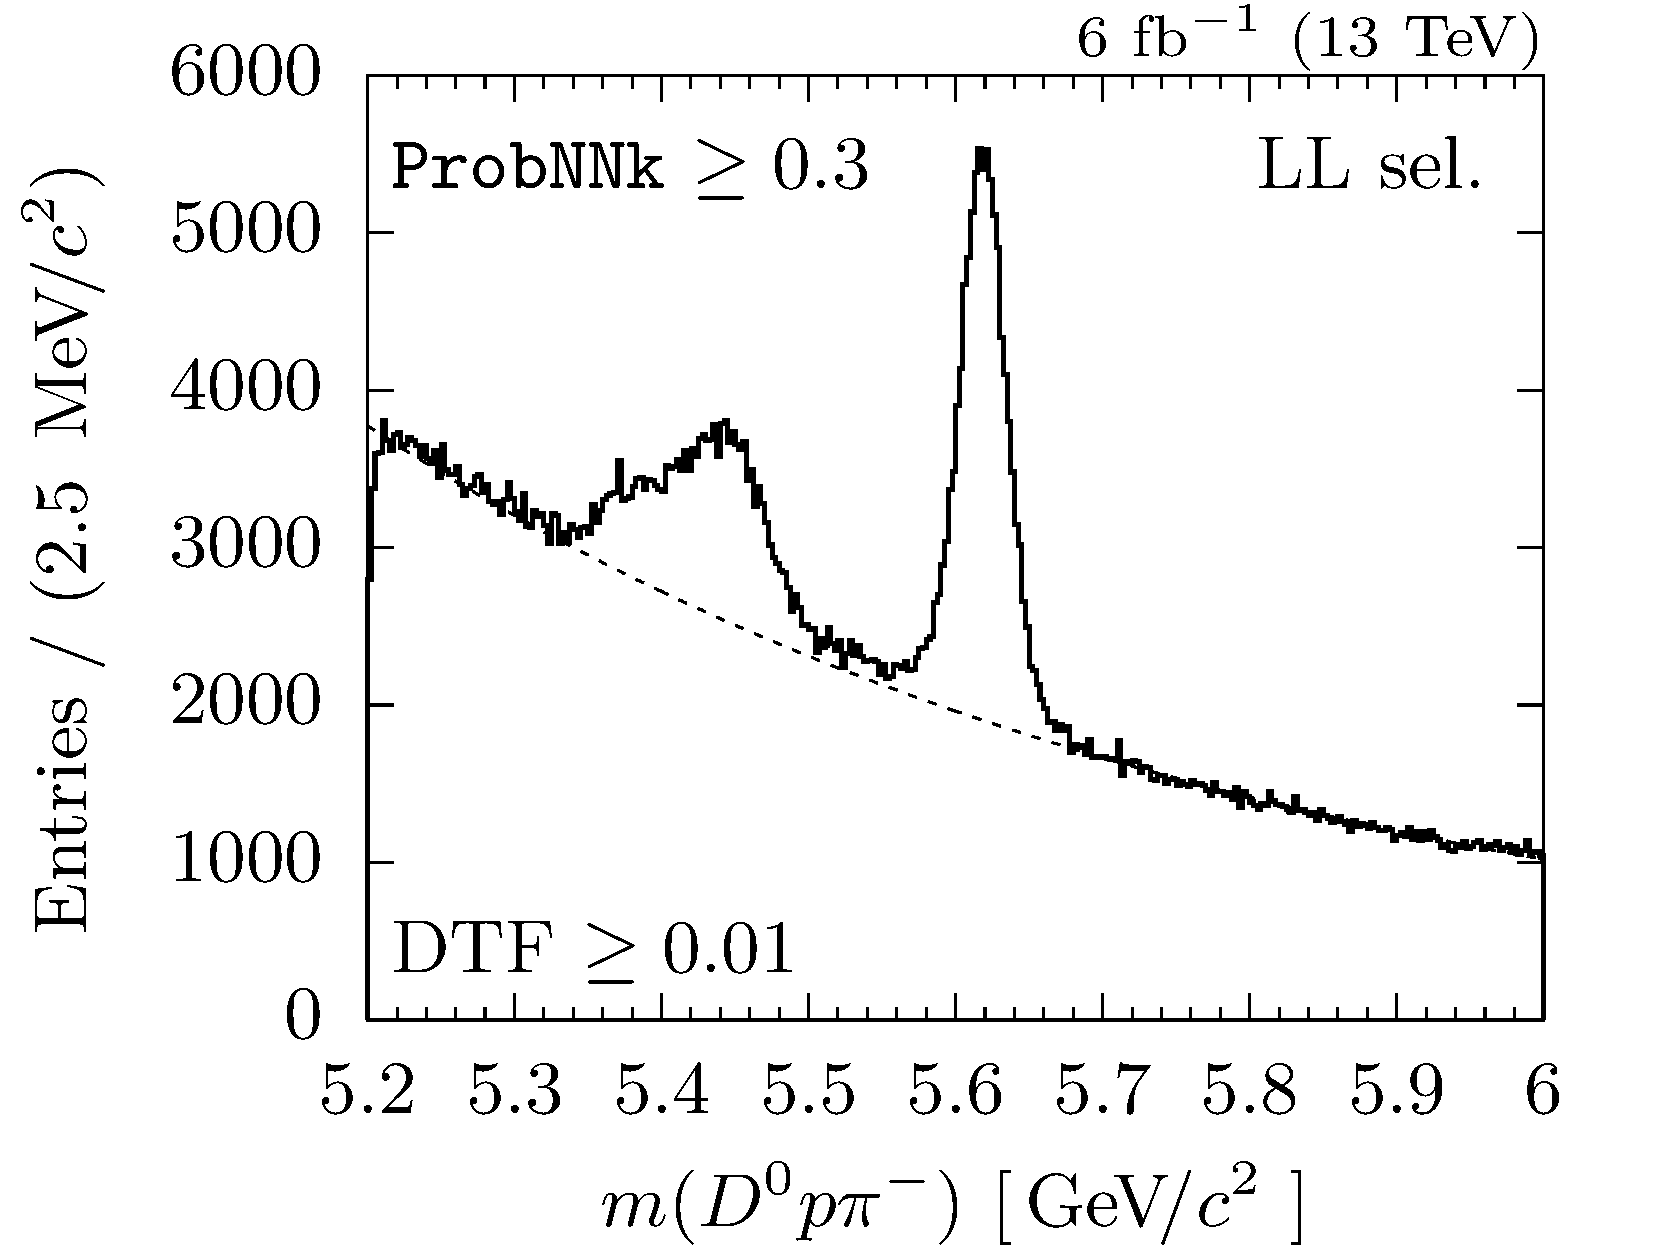
\includegraphics[scale=1.]{Lb2Dzppi_mvaxcheck/hLbM_LL_no_clf.png}
    \end{subfigure}
    \begin{subfigure}{.49\textwidth}
        \centering
        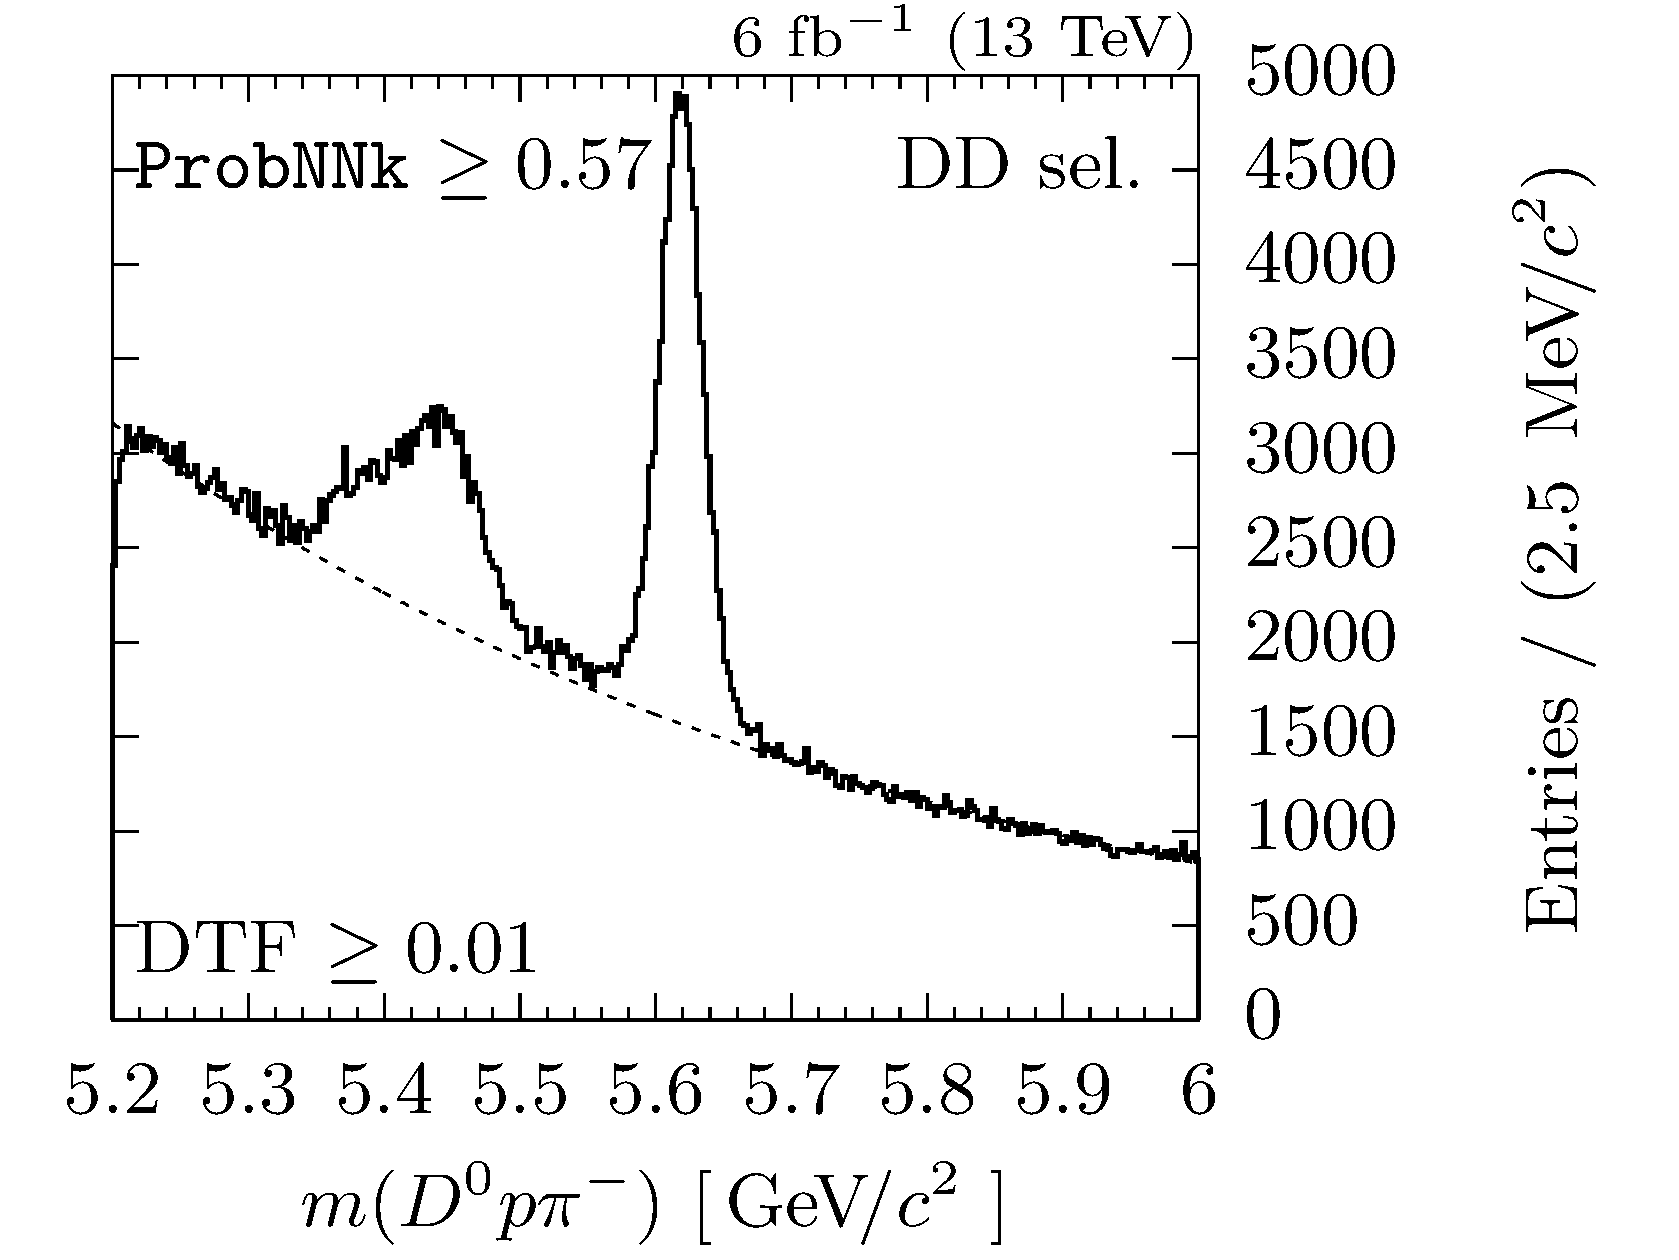
\includegraphics[scale=1.]{Lb2Dzppi_mvaxcheck/hLbM_DD_no_clf.png}
    \end{subfigure}
    \caption{Combined invariant mass distributions of \Dz, \proton and \pim candidates, as well as the fit of the combinatorial background (dashed line). The distributions are the result of a set of selection criteria that resembles part of the tight selection for \gls{LL} (left) and \gls{DD} (right) \decay{\Lb}{\Dz\Lz} decays.}
    \label{fig:LbToDzppi_hLbM_no_clf}
\end{figure}

Requiring both of these selection criteria results in a cleaner data sample but also unveils a bias of the fit model at the lower tail of the \Lb signal peak.
The fitted yields of these two fits are shown in Tab.~\ref{tab:LbToDzppi_xcheckN}.
Applying the very same fitting strategy to \gls{mc} simulated events gives access to the (\gls{mc} predicted) efficiency of the required selection and allows the extrapolation to the total amount of events before requiring the selection.
Both of these extrapolated numbers should match the number we found with our first fit.
The deviation is an admixture of deviations due to fidelity issues of the \gls{mc} simulated events and an overestimation of the signal yield due to a bias of the fitting model.
A conservative approach to approximate the systematic uncertainty of the fit is to ignore the former part and take the entire deviation between the three fitted yields as an upper limit of the uncertainty interval,
\begin{equation*}
    n = 7.0(5) \times 10^4 \,.
\end{equation*}
The uncertainty corresponds to a relative uncertainty of $7\,\%$ which is sufficient for the sake of the present analysis.
As stated, this approximation is conservative and renders additional studies, such as the unfolding of the strongly correlated systematic uncertainties of the three samples, unnecessary.
\begin{table}[htbp]
    \centering
    \caption{Efficiencies of applying additional selection criteria (\gls{LL}~sel.) and (\gls{DD}~sel.) on top of the loose selection of \decay{\Lb}{\Dz\proton\pim} decays, evaluated by fitting \gls{mc} simulated events. These efficiencies are then used to extrapolate (ext.) the fitted yields (fit~2) of recorded data and compared with the fitted yield (fit~1) of the respective distribution after requiring only the loose selection.}
    \label{tab:LbToDzppi_xcheckN}
    \begin{tabular}{lll}
        \toprule
        & \multicolumn{1}{c}{\gls{LL} sel.} & \multicolumn{1}{c}{\gls{DD} sel.} \\
        \midrule
        %MC efficiency & $77.009(34)\,\%$ & $71.77(4)\,\%$ \\
        %ec.\ data (fit 2) & $5.776(34) \times 10^4$ & $5.282(32) \times 10^4$ \\
        %ec.\ data (ext.) & $7.50(4) \times 10^4$ & $7.36(4) \times 10^4$ \\
        \gls{mc} efficiency & $77.020(34)\,\%$ & $71.70(4)\,\%$ \\
        Rec.\ data (fit 2) & $5.746(34) \times 10^4$ & $5.301(32) \times 10^4$ \\
        Rec.\ data (ext.) & $7.45(4) \times 10^4$ & $7.39(4) \times 10^4$ \\
        \midrule
        %Rec.\ data (fit 1) & \multicolumn{2}{c}{{$7.07(6) \times 10^4$}} \\
        Rec.\ data (fit 1) & \multicolumn{2}{c}{{$7.04(6) \times 10^4$}} \\
        \bottomrule
    \end{tabular}
\end{table}

In Chap.~\ref{chap:br} we argue that only events with a positive \gls{lzero} \gls{tis} trigger decision are needed for the normalization of the branching ratio.
The corresponding distributions of the invariant mass $m(\Dz\proton\pim)$ and the respective fits for recorded data are shown in Fig.~\ref{fig:LbToDzppi_hLbM_no_clf_tis}.
The fits yield (including our $7\,\%$ uncertainty estimation) $n = 3.93(28) \times 10^4$ and $n = 3.60(25) \times 10^4$ for the \gls{LL} and \gls{DD} selection, respectively.
\begin{figure}[htbp]
    \centering
    \begin{subfigure}{.49\textwidth}
        \centering
        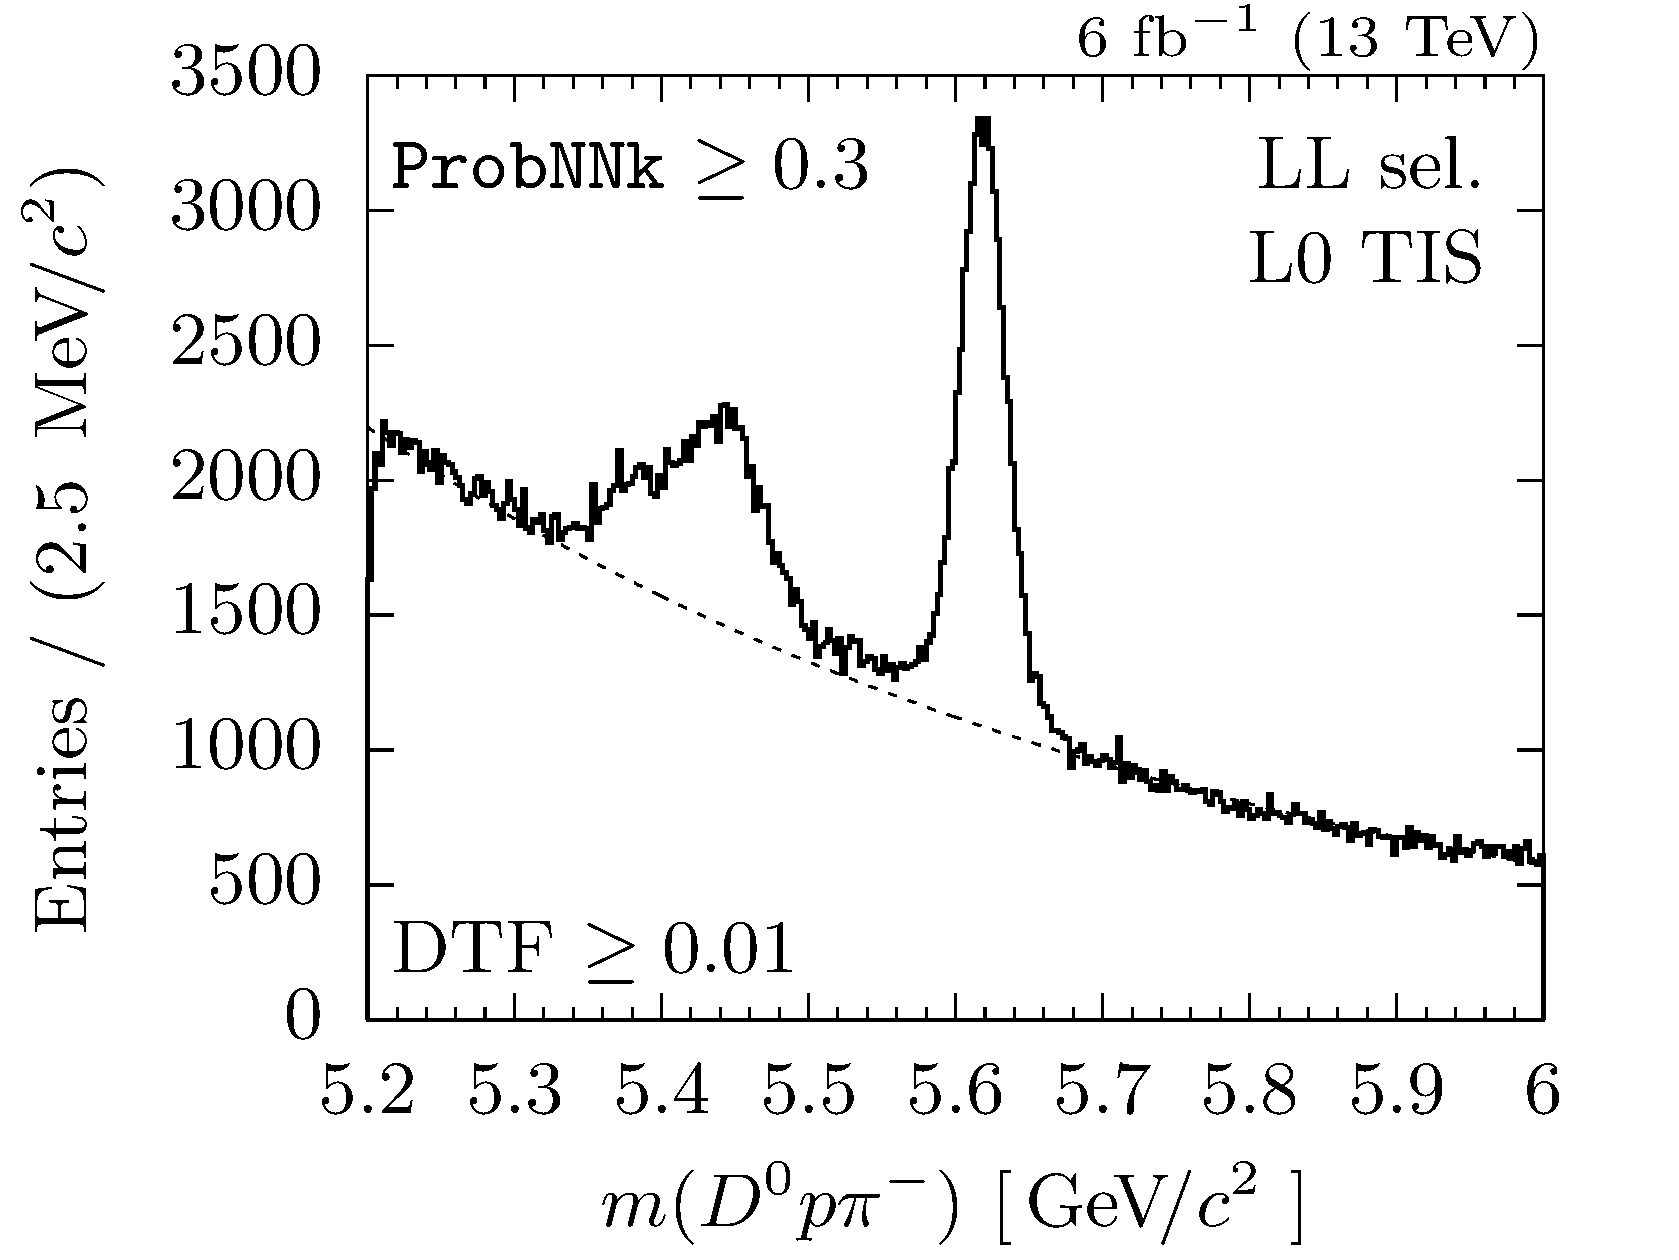
\includegraphics[scale=1.]{br/hLbM_LL_no_clf_tis.png}
    \end{subfigure}
    \begin{subfigure}{.49\textwidth}
        \centering
        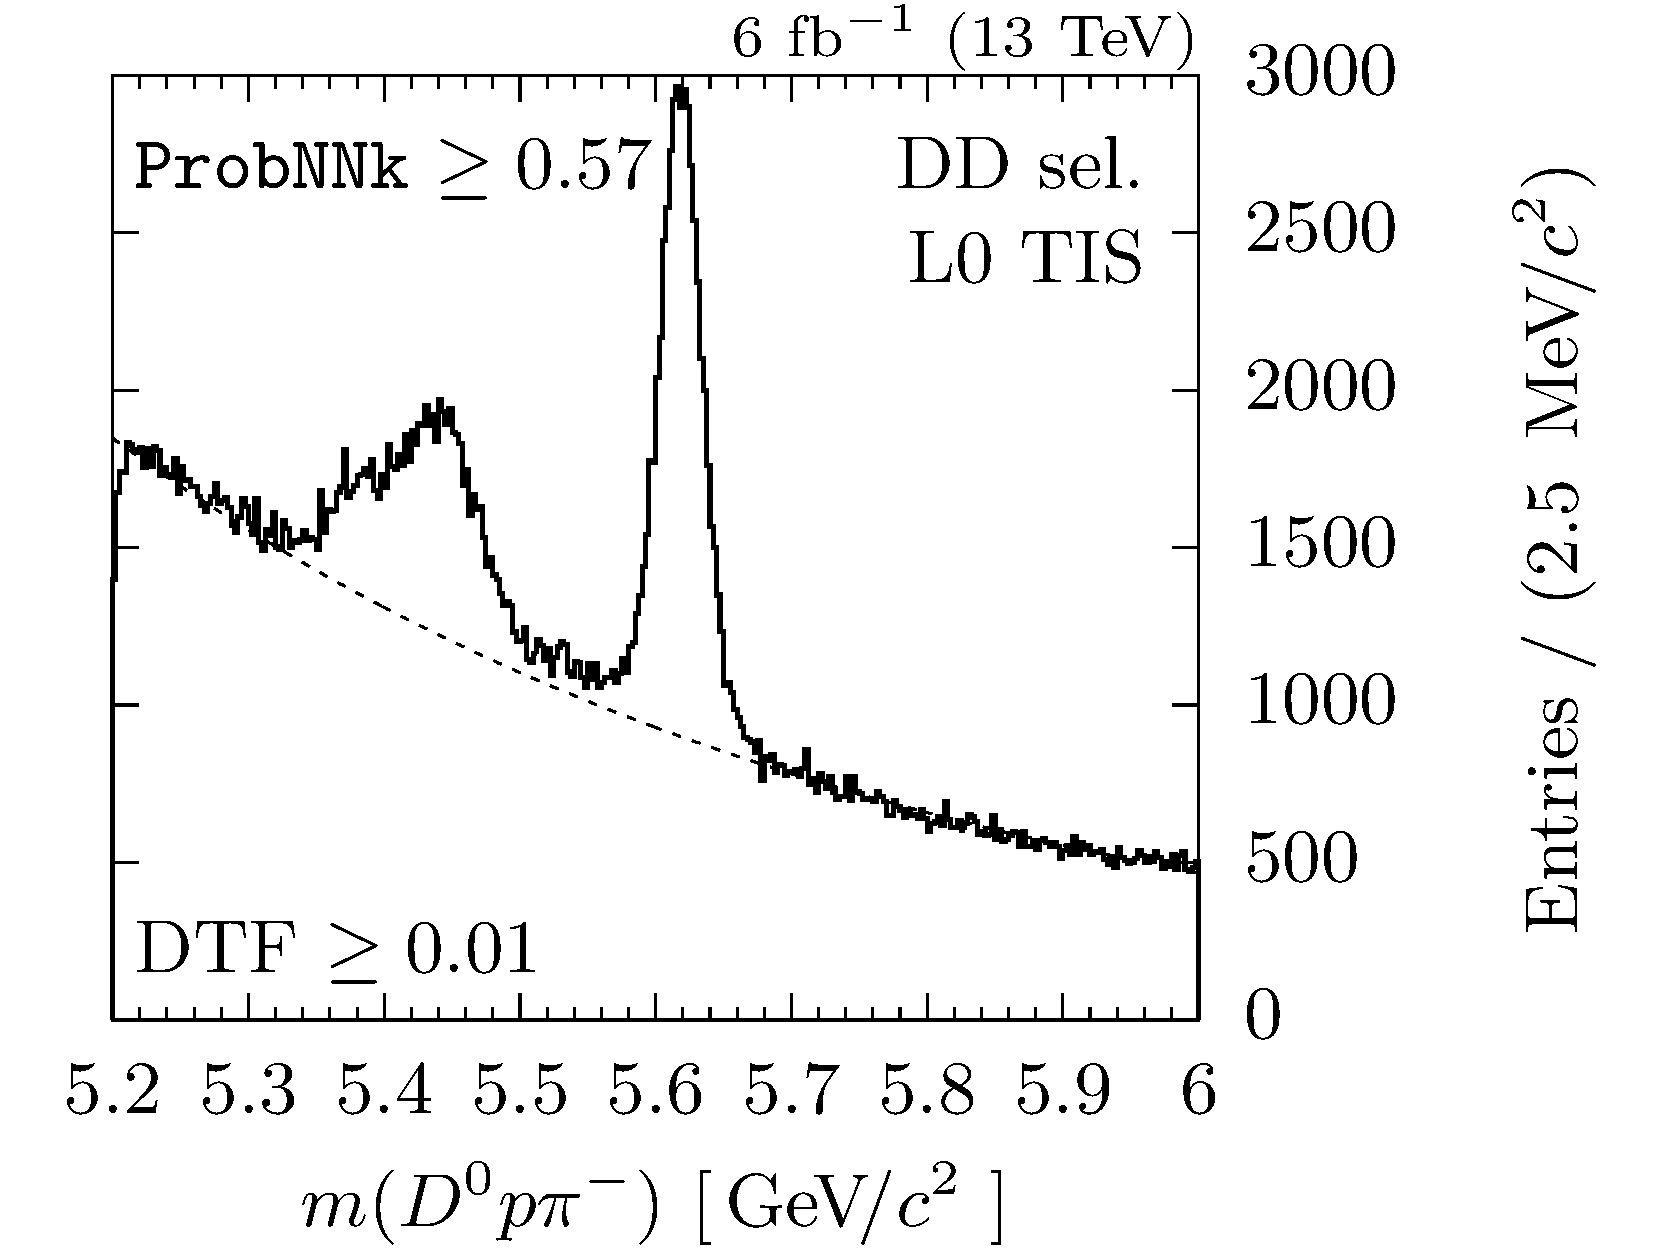
\includegraphics[scale=1.]{br/hLbM_DD_no_clf_tis.png}
    \end{subfigure}
    \caption{Combined invariant mass of \Dz, \proton and \pim candidates from recorded data. The selection criteria resembles parts of the tight selection for \gls{LL} (left) and \gls{DD} \decay{\Lb}{\Dz\Lz} decays. Additionally, the \gls{lzero} \gls{tis} trigger is required.}
    \label{fig:LbToDzppi_hLbM_no_clf_tis}
\end{figure}

